\subsection{The Relay}
	A relay is a device that acts as an electromechanical switch, it consists of three basic parts: a coil, a set of contacts and a reset spring as shown in Figure \ref{fig-relay}. When an electric current flows through the coil, this creates a magnetic flux that changes the state of the set of contacts thus changing the position of the switch. When the coil is de-energized the reset spring returns the key to its natural state. The relays are used for various applications in the automotive industry, because a relay allows two circuits to interact without there being an electric current transfer between them, in this way smaller power circuits can control higher current circuits and vice versa \cite{keller1962relays} .

	\begin{figure}[htbp]
		\centering
			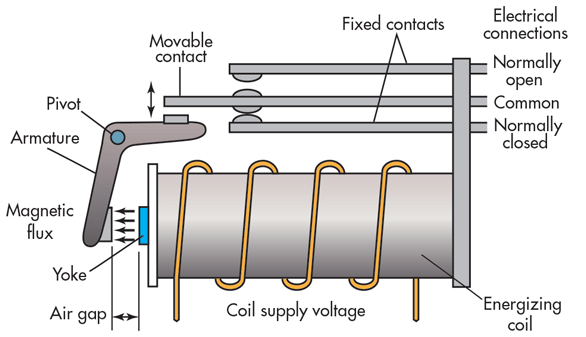
\includegraphics[scale=0.45]{figuras/fig-relay.png}
			\caption{Esquemático Relê \cite{relay-scheme}}
		\label{fig-relay}
	\end{figure}
